% ---------------------------------------------------------------- main text: architecture only
\begin{figure}[htbp]
    \centering
    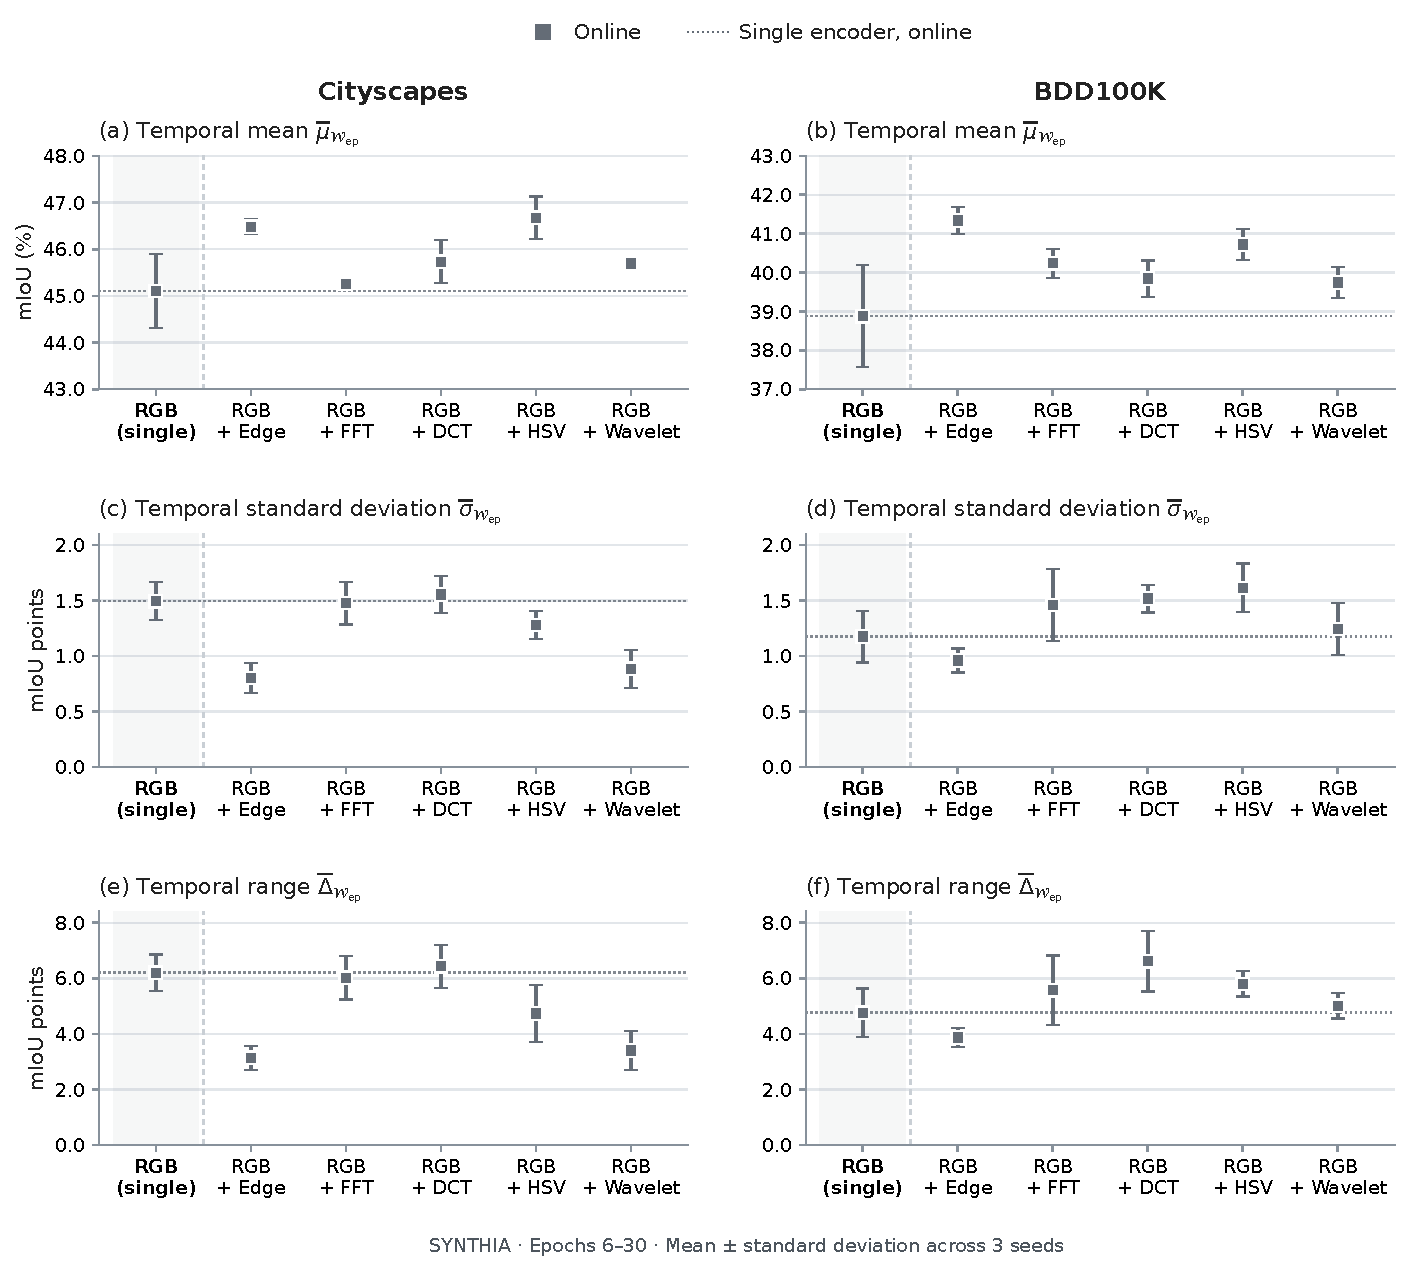
\includegraphics[width=\textwidth]{figures/synthia_dual_adaptive_temporal_online.pdf}
    \caption[SYNTHIA results: adaptive bidirectional dual encoder without EMA]{%
    \textbf{Temporal target-domain performance of the adaptive bidirectional
    dual-encoder model compared with the single-encoder model for SYNTHIA
    training.}
    Only online parameters are shown; metrics are computed over epochs
    $6$--$30$. \emph{RGB + view} denotes the dual-encoder model with the
    corresponding auxiliary view. The dotted line indicates the
    single-encoder performance. Markers indicate the mean across three
    seeds; vertical bars indicate the corresponding standard deviation.
    Single-encoder results use the same three seeds and therefore differ
    slightly from Section~\ref{sec:results_single_ema}. Complete results and
    trajectories are provided in
    Tables~\ref{tab:synthia_dual_adaptive_windows_cityscapes}
    and~\ref{tab:synthia_dual_adaptive_windows_bdd} and
    Figure~\ref{fig:synthia_dual_adaptive_trajectories}.}
    \label{fig:synthia_dual_adaptive_online}
\end{figure}

% ---------------------------------------------------------------- main text: combined with EMA
\begin{figure}[htbp]
    \centering
    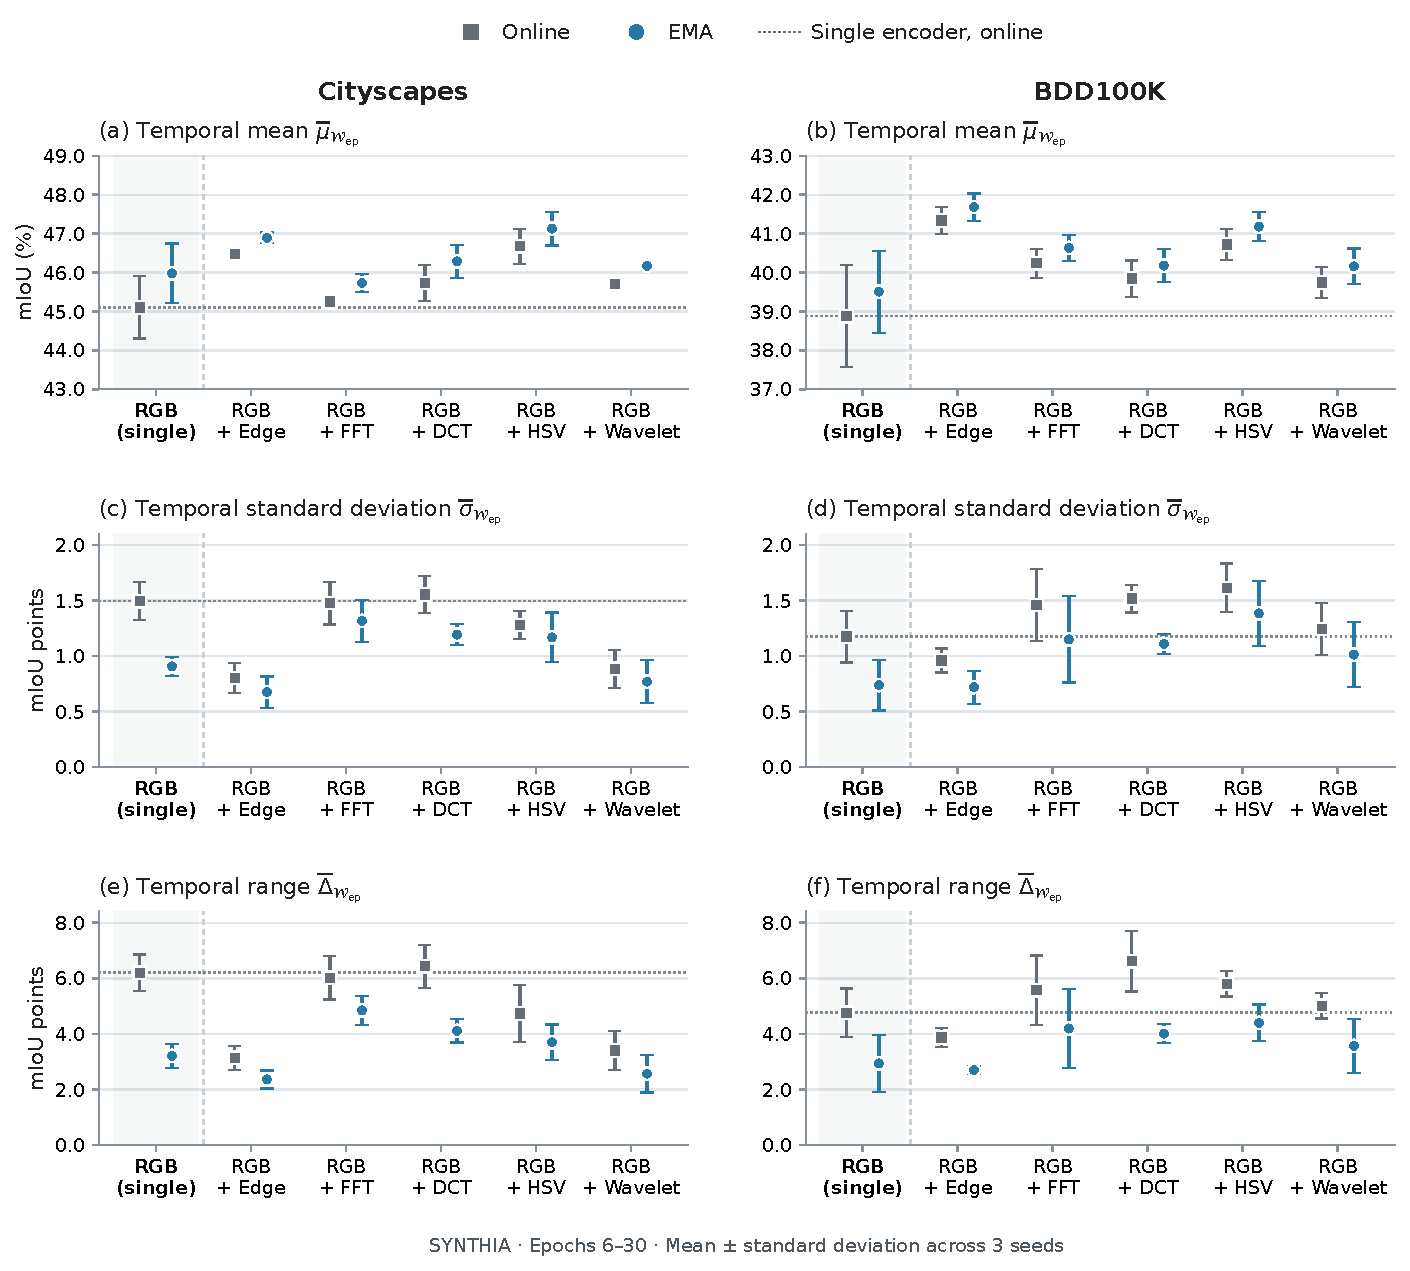
\includegraphics[width=\textwidth]{figures/synthia_dual_adaptive_temporal_online_ema.pdf}
    \caption[SYNTHIA results: adaptive bidirectional dual encoder with and without EMA]{%
    \textbf{Combined effect of dual-encoder processing and EMA for the
    adaptive bidirectional variant and SYNTHIA training.}
    Online (squares) and EMA parameters (circles) are shown for the
    single-encoder model and each dual-encoder variant; metrics are computed
    over epochs $6$--$30$. \emph{RGB + view} denotes the dual-encoder model
    with the corresponding auxiliary view. The dotted line indicates the
    online performance of the single-encoder model. Markers indicate the mean
    across three seeds; vertical bars indicate the corresponding standard
    deviation. EMA uses the reference configuration ($\lambda=0.995$, $u=20$).
    Complete results and trajectories are provided in
    Tables~\ref{tab:synthia_dual_adaptive_windows_cityscapes}
    and~\ref{tab:synthia_dual_adaptive_windows_bdd} and
    Figure~\ref{fig:synthia_dual_adaptive_trajectories}.}
    \label{fig:synthia_dual_adaptive_online_ema}
\end{figure}

% ---------------------------------------------------------------- appendix: trajectories
\begin{figure}[htbp]
    \centering
    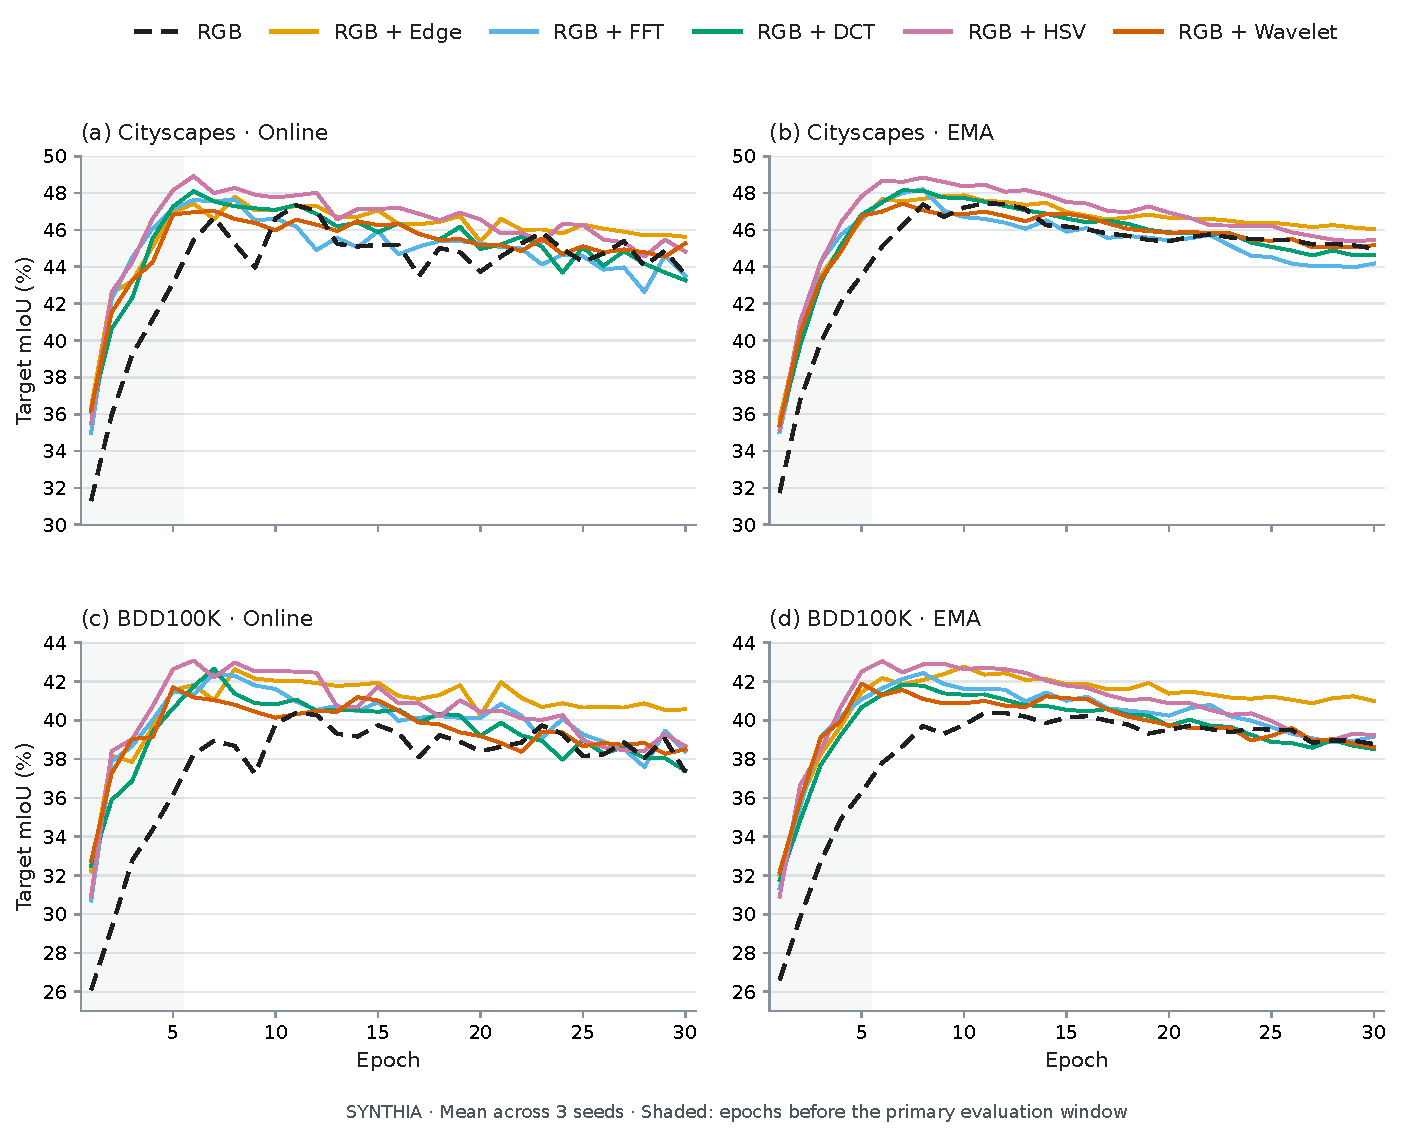
\includegraphics[width=\textwidth]{figures/synthia_dual_adaptive_trajectories.pdf}
    \caption[SYNTHIA results: trajectories of the adaptive bidirectional dual-encoder variants]{%
    \textbf{Target-domain performance trajectories of the adaptive bidirectional
    dual-encoder variants for the SYNTHIA-trained models.}
    Lines show the mean target-domain mIoU across three seeds for online
    (left) and EMA parameters (right) on Cityscapes (top) and BDD100K
    (bottom). The single-encoder model (\emph{RGB}) is shown as a dashed
    reference; \emph{RGB + view} denotes the dual-encoder model with the
    corresponding auxiliary view. The shaded region marks the epochs
    preceding the primary evaluation window. EMA uses the reference
    configuration ($\lambda=0.995$, $u=20$). The corresponding temporal
    metrics are reported in
    Tables~\ref{tab:synthia_dual_adaptive_windows_cityscapes}
    and~\ref{tab:synthia_dual_adaptive_windows_bdd}.}
    \label{fig:synthia_dual_adaptive_trajectories}
\end{figure}
